\section{Méthodologies}

\subsection{Gestion de la bibliographie}
Pour la gestion de la bibliographie au sein du document,
nous utilisons le package \texttt{biblatex}.
Celui-ci permet d'écrire l'ensemble de nos références dans un fichier \texttt{.bib}
sous la forme suivante.
\begin{verbatim}
  @online{histoire_mod_plantes,
    title = {Une histoire de la modélisation des plantes},
    author = {Philippe de Reffye and Marc Jaeger 
    and Paul-Henry Cournède},
    url = {https://interstices.info/jcms/c_38032/une-histoire-de-
    la-modelisation-des-plantes},
    year = {2009},
    month = "04",
  }
\end{verbatim}
La mise en page est alors automatique en fonction des informations fournies
et le rendu de l'exemple est présenté ci dessous.
\begin{figure}[h]
  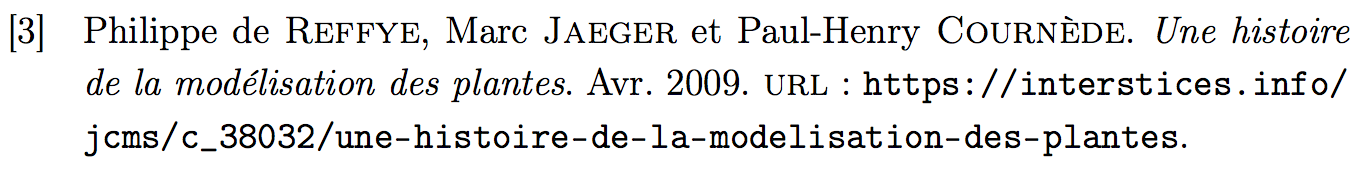
\includegraphics[scale=0.6]{./img/rendu_elem_bib.jpg}
\end{figure}

Cela parait à priori assez lourd d'écrire soi-même toutes les informations
en suivant cette syntaxe mais il existe des logiciels comme Zotero
qui font le travail à notre place.
Les sources trouvées sur Google Scholar peuvent également être exportées
aisément au format \texttt{BibTex}.


\subsection{Outils de travail collaboratif}
Pour des raisons pratiques et esthétiques, nous avons décider d'écrire
nos rapports en \LaTeX{}.
Il s'agissait donc de trouver la meilleure façon de partager le code source
et de pouvoir contrôler les changements apportés au document.
Une première idée pourrait être d'utiliser ShareLaTeX qui propose une plate-forme
de compilation en ligne ainsi qu'un système de gestion de versions
assez simple à utiliser.
Nous n'avons pas choisi cette solution notamment pour les raisons suivantes.
L'utilisateur doit être connecté dès qu'il veut travailler sur le projet,
le système de compilation est assez lent et l'utilisateur n'est pas libre
d'utiliser son éditeur de texte ou son visualisateur de \textsc{pdf} favori.

Pour palier aux problèmes décrits ci-dessus, le logiciel \texttt{git}
associé à GitHub est une très bonne alternative.
Il permet en effet à chaque membre du groupe de travailler sans être connecté
ainsi que d'utiliser son éditeur et compilateur favori.
Chaque membre travaille donc de son côté en faisant des \emph{commits}
et lorsqu'il juge que son travail est utile pour les autres, 
il \emph{push} sur le serveur.
L'algorithme du fusion, \emph{merge}, permet également de fusionner intelligemment
les lignes d'un fichier qui ont été modifiées par plusieurs membres.
Le dernier point à souligner est que \texttt{git} permet une gestion des branches,
particulièrement pratique lorsqu'on veut développer une partie du projet
sans risquer de créer des erreurs dans le programme principal.

Nous combinons donc ces deux outils pour 
\begin{enumerate}
  \item implémenter le modèle LNAS blé dans la plateforme
  Pygmalion en \textsc{Julia} (une description plus détaillée de
  l'objectif attendu pour cette partie est décrite dans la
  section~\ref{sec:contexte} à la page~\pageref{sec:contexte})
  pour le client dont le code source est sur la plateforme GitLab,
  \item rédiger l'étude documentaire en partageant le code \LaTeX{}
  à l'aide d'un dossier sur 
  GitHub\footnote{\url{https://github.com/jdewasseige/projet-sbt11}}.
\end{enumerate}

\subsection{Organisation et partage des tâches}
Il nous reste un dernier point à décrire, celui de la \emph{communication}
au sein du groupe.
Nous utilisons Slack\footnote{\url{https://slack.com/}} qui est un logiciel
de plus en plus utilisé pour les travaux de groupe ainsi que dans les start-ups.
Il permet d'éviter de devoir alterner entre plusieurs applications comme les mails,
DropBox et Twitter, puisqu'il permet d'être connecté
à celles-ci au sein de l'application.
On peut également créer plusieurs \emph{channels} pour séparer la communication
entre les différentes tâches.
Par exemple dans ce projet nous avons les \emph{channels} suivantes :
\texttt{general}, \texttt{etude-documentaire}, 
\texttt{planning} et \texttt{dev\_plate-forme}.
On trouve aussi un système d'historique et de gestion de fichiers efficace.

L'ensemble des tâches ainsi que leur répartition pendant l'année
est associé au planning \textsc{Gantt} qui se trouve
dans l'Annexe~\ref{ann:planning} à la page~\pageref{ann:planning}.
